\documentclass[11pt]{report}

% Two-sided draft --- doesn't allow for binding room
%\usepackage[a4paper,twoside,left=35mm,right=35mm,top=40mm,bottom=35mm]{geometry}
% Two-sided final --- uneven margins to allow for binding
\usepackage[a4paper,twoside,left=35mm,right=25mm,top=40mm,bottom=35mm]{geometry}

% This line prevents LaTeX complaining about \headheight being too small.
\setlength{\headheight}{15pt}
\usepackage{inputs/masthesis}

% One-and-a-half or double-line spacing.  I used 1.5 for final submission.
\onehalfspacing
%\doublespacing

\begin{document}

  \phdtitle{Collective Behaviour}
           {Jack Walton}
           {March 2020}

  \thispagestyle{empty}
  \cleardoublepage

  %\begin{dedication}
  Add a dedication here if you wish.
\end{dedication}
\thispagestyle{empty}
\cleardoublepage


  %\thispagestyle{empty}
\clearpage

\vspace*{\stretch{2}}

\begin{center}
  \textbf{Acknowledgements}\\[0.75cm]

  \begin{minipage}{0.9\textwidth}
    \setlength{\parskip}{0.45em}

    This thesis wouldn't have been possible without the saintly patience of my
    supervisors Andrew Baggaley, Andrew Fletcher and Colin Gillespie, who were
    tasked with the unenviable job of keeping me on-topic. Thank you for your
    guidance, expertise, and endless creative flair in getting me out of
    faculty workshops and the dreaded ``MAGIC'' lecture series.

    Within the department I'd like to thank my friends and office-mates for
    their unwavering companionship and \emph{insatiable} desire for distraction
    and procrastination. I must also express my gratitude to Michael Beaty and
    George Stagg for helping with my (sometimes sensible) computing requests.

    Of course it is only with the financial support of EPSRC that my last few
    years of study have been viable. So, EPSRC, if you're reading this: thank
    you.

    Lastly, dear reader, thank you for your keen eye for typographical detail,
    and for looking at the pictures, but not reading the text too closely\ldots
  \end{minipage}

\end{center}

\vspace*{\stretch{3}}

\cleardoublepage


  %\thispagestyle{empty}

\clearpage

\vspace*{\fill}

\begin{center}
  \textbf{Abstract}\\[0.75cm]

  \begin{minipage}{0.9\textwidth}
    \setlength{\parskip}{0.45em}

    The study of collective behaviour---broadly defined as the formation of
    macro-level structures from the interactions between individuals---has in
    recent years become a thriving topic of multi-disciplinary research. Under
    consideration of biological-fitness the scientist has been able to reason
    about \emph{why} these structures form, and the advantages which the
    collective can afford the individual. However, much less is known about
    \emph{how} these structures are formed and maintained in the first place.

    Much work has been invested in the development of mathematical models which
    seek to explain the formation and maintenance of animal aggregations.
    Research has shown that behaviour reminiscent of real flocking events can
    arise from simple mathematical models which describe how individuals
    interact with one another. However, much of this modelling relies on
    aprioristic assumptions about how individuals behave and interact, with
    little-to-no verification against real observation.

    In this work we examine mathematical models popular in the literature and
    suggest modifications motivated by considerations of biological-realism. In
    particular we advocate adoption of continuous interaction rules, and
    consider how behavioural and biological variation can be accounted for by
    imposing hierarchical structure.

    We proceed to fit these models of collective behaviour to observations of
    real and simulated flocking events. Model fitting is performed in a
    Bayesian framework, allowing the quantification of parameter uncertainty.
    Fitting models to simulated data provides opportunity to assess the
    effectiveness and accuracy of our inference schemes, before attempting the
    same inference on real observation. Multiple competing models are fit to
    the same data, with the predictive performance of these models ranked using
    ideas from the model-selection literature. We are then able to recommend a
    subset of the candidate models as providing the best performance.

    Finally, consideration is made for datasets which exhibit missing
    observations. Such missingess occurs naturally owing to the fixed-location
    recording equipment used to capture flocking events. We argue that this
    missingness \emph{cannot} be ignored, and that it must be accounted for
    during any model-fitting process. Techniques are outlined which allow the
    researcher to account for missingness. Simulation studies are performed
    which demonstrate the efficacy of the proposed approach, before these
    techniques are demonstrated on a real dataset exhibiting missingness.

  \end{minipage}

\end{center}

\vspace*{\fill}

\cleardoublepage


  \pagenumbering{roman}                 % Change the page numbering style for

  \microtypesetup{protrusion=false} % disables protrusion locally in the document
  \tableofcontents
  \microtypesetup{protrusion=true} % enable protrusion

  %\listoffigures

  %\listoftables

  \clearpage                            % End the current page making sure all
  \thispagestyle{empty}                 % tables/figures are printed.
  \cleardoublepage                      % Necessary for correct page numbering.

  \pagenumbering{arabic}                % Reset the page numbering style.

  %\part{Title of My First Part}

  \chapter{Introduction}
\label{cha:introduction}

\section{Motivation}
\label{sec:motivation}

Many of us have been struck by the inherent beauty of animals moving collectively; starlings gathering at dusk in huge numbers to perform the most mesmerising of ballets, the entire flock moving as if some fluid object; fish forming tight milling structures in defence against predation, changing direction in the blink of an eye and with a flash of silver. At different length scales, and in both the living and non-living domains, startling examples of collective behaviours have been observed.

\begin{figure}[!htbp]
	\centering
	\includegraphics[width=\textwidth]{fig/murmuration.jpg}
	\caption{A particularly startling example of a starling murmuration, captured near Gretna in the Scotish Borders. Photograph: Owen Humphreys/PA.}
	\label{fig:murmuration}
\end{figure}

Over the years collective behaviour has become a thriving topic of multidisciplinary research, capturing the imaginations of physicists, biologists, mathematicians and statisticians. Our understanding has evolved significantly from early suggestions that collective behaviour results from thought-transference and telepathy between individuals \citep{selous31}. Though we can often explain why animal aggregations are evolutionary advantageous, little is in fact known about how these structures are formed in the first place.

Much work has been invested in developing theoretical models which seek to explain emergent behaviour by interactions at an individual level. Such models have shown that individual interactions are sufficient to produce group-level structures. Many different simulations, implementing disparate interaction rules, are able to produce behaviour reminiscent of real flocking systems. However, these models have largely only been verified with comparison to empirical observation at a qualitative level, and a thorough quantitative comparison between field data and theory has been lacking.

In recent years technological and methodological advances have made it possible to capture the movements of large groups of animal aggregates. With this data, it is only now that we are in a position to make a robust comparison between model predictions and real-world observations.

In this thesis we utilise real data to perform statistical inference on theoretical models. Our inference is made in a Bayesian framework. Bayesian inference allows the capture of uncertainty about fitted model parameters, flexible model structures and potential inclusion of expert information via the prior distribution. With this we seek to fit empirical data to a generalisation of a popular model from the literature.

\section{Biological Function}
\label{sec:biological_function}

\color{red} In which I plan to discuss the `why' of collective behaviour. That is, to discuss the evolutionary advantages which aggregations offer individuals. \color{black}

\section{Theoretical Models}
\label{sec:models}

Models of collective behaviour can largely be divided into two classes: Lagrangian and Eulerian. These descriptions are analogous to the models of fluid dynamics, where Lagrangian models consider the flow in terms of interactions of fluid parcels and Eulerian models consider the changing fluid properties at a given point in space and time. In the context of collective behaviour Lagrangian models simulate the movements of interactions and Eulerian models typically model the density of a group through space and time.

\subsection{Lagrangian Models}
\label{ssec:lagrangian_models}

So called agent-based models (ABMs), also referred to as Lagrangian models, have proven a useful tool in modelling collective behaviours. In these models the behaviour of an agent is modelled at the individual level. An agent's behaviour is determined by social interactions with neighbouring individuals. Examples of typical interactions include the desire to move in the same direction as neighbours (alignment, or orientation), the desire to avoid collisions (repulsion) and a desire to remain close to neighbours (attraction). Along with specifying social behaviours ABMs suggest methods by which agents identify neighbours to interact with. An individual may identify neighbours as; within a certain distance; positioned inside a field of vision or as one of a fixed number of closest agents.

In a pioneering paper, \citet{aoki82} developed an ABM to simulate the movements of schooling fish in two-dimensions. Here it was shown that collective behaviour can arise from simple interactions at an individual level and without the need of a leader. The model simulated zonal interactions in which the area around an individual is partitioned into zones of repulsion, alignment and attraction. The partitioning of space in this way is illustrated in Figure \ref{fig:zone_illustration}. As well as zonal interactions this model accounted for fish having incomplete fields of vision. Further models were also devised to simulate fish schools \citep{okubo86, huth92}.

\begin{figure}
	\centering
	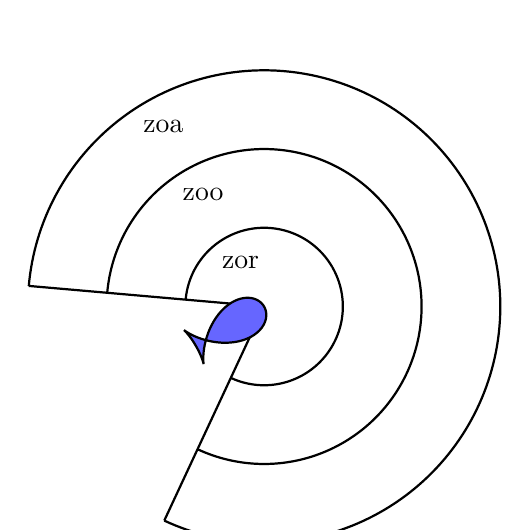
\begin{tikzpicture}[rotate=30]
	   \draw [thick, domain=0:145, samples=100] plot ({cos(\x)}, {sin(\x)});
	   \draw [thick, domain=215:360, samples=100] plot ({cos(\x)}, {sin(\x)});
	   \draw [thick, domain=0:145, samples=100] plot ({2*cos(\x)}, {2*sin(\x)});
	   \draw [thick, domain=215:360, samples=100] plot ({2*cos(\x)}, {2*sin(\x)});
	   \draw [thick, domain=0:145, samples=100] plot ({3*cos(\x)}, {3*sin(\x)});
	   \draw [thick, domain=215:360, samples=100] plot ({3*cos(\x)}, {3*sin(\x)});
	   \draw [thick] (0, 0) -- ({-3*sin(270-145)}, {-3*cos(270-145)});
	   \draw [thick] (0, 0) -- ({3*sin(145-200)}, {-3*cos(145-200)});
	   % make that sweet sweet fish curve
	   \draw [fill=blue!60!white, thick, domain=-200:200, samples=100] plot ({0.5*(cos(\x) - sin(\x)^2/1.41)-0.5}, {0.5*sin(\x)*cos(\x)});
	   \node [text width=1cm] at (0.25, 0.5) {zor};
	   \node [text width=1cm] at (0.25, 1.5) {zoo};
	   \node [text width=1cm] at (0.25, 2.5) {zoa};
	\end{tikzpicture}
	\caption{An illustration of the area around an agent partitioned into multiple zones. zor: zone of repulsion, zoo: zone of orientation (or alignment), zoa: zone of attraction. The missing segment behind the agent represents the blind zone in which it cannot see.}
	\label{fig:zone_illustration}
\end{figure}

\citet{reynolds87} formulated a theoretical model, motivated by the production of computer animations, which described the movement of flocking birds in three-dimensional space. To produce more aesthetically pleasing animations, the software, ``Boids'', included sophistications such as banking during turns. This focus on developing simulations which produce elegant behaviour made rigorous scientific analysis difficult. Interestingly, Tim Burton's 1992 Batman Returns used a modified version of the Boids software to simulate animations of bat swarms and penguin flocks.

Motivated by research within statistical physics, \citet{vicsek95} introduced a simple two-dimensional model in which self-propelled particles move with a fixed absolute velocity and align with neighbours within an interaction zone. This model is commonly referred to as ``Vicsek Model" (VM), which we shall later use to formulate our ``Generalised Vicsek Model" (GVM). Despite its simplicity this model produces complex-behaviour resembling that of a real biological system. Vicsek et al. investigated the phase transition between ordered and disordered motion as the density of particles and noise in the system varied.

Later, models were developed to explore the movements of mammals and other vertebrate groups. \citet{couzin02} showed major group-level behavioural changes as minor changes in individual interaction rules were made. With small changes in the model parameters, groups transitioned from disordered, swarm like behaviour, to toroidal milling structures, to forming dynamic and highly parallel groups. Further research was made by \citet{couzin05} which investigated how leaders influence the motion of travelling groups. This work showed that only a small proportion of leaders are necessary to guide groups with a high degree of accuracy. Further results investigated how groups of individuals make collective decisions in the face of conflicting desires.

As a method for exploring collective behaviour, Lagrangian models are very appealing in their intuitiveness and in the ease of implementing explicit behavioural rules. Though for many years the simulation and exploration of these models was limited by computing power; modern computation allows for the simulations of large groups over many time steps. With these advances in computing, and a growing interest in the field, a significant proportion of the literature focuses on the analysis and exploration of agent-based models.

\subsection{Eulerian Models}
\label{ssec:eulerian_models}

Sometimes known as continuum models, Eulerian models are complementary to the Lagrangian method. This approach describes a group by the density of organisms at a point in space. Eulerian models are typically constructed of a set of partial differential equations which describe how density develops over time.

One such Eulerian approach by \citet{gueron93} modelled the movements of large groups of wildebeests. The predictions of the model were compared with aerial observations of migrating wildebeest in the Serengeti. The large-scale front patterns seen in the aerial photography were reproduced by the model.

Eulerian models have also been used to analyse vortex solutions \citep{topaz04} and stationary clump solutions \citep{topaz06}.

However, the Eulerian approach is limited. Most analyses are restricted to 1-dimension and the approach has not proven appropriate for modelling groups of low densities. With this in mind, and with the advantages of the Lagrangian approach, in this thesis we will concentrate entirely on modelling in the Lagrangian framework.

\section{Empirical Studies}
\label{sec:empirical_studies}

Real data of animal aggregations is essential to ensure that theoretical models are falsifiable. The emergence of a desired pattern from simulation is not sufficient evidence that a model is correctly capturing the interactions of individuals. This observation is further compounded by the understanding that models employing different local interactions can produce similar looking behaviour at the group level.

Thorough comparison between real data and model predictions have proven difficult largely because of the scarcity of appropriate data. The collection of suitable data can be a complicated and convoluted process. Taking observations in the field is technically demanding, requiring the precise calibration of sensitive measurement equipment, not to mention the additional difficulty of the typically three-dimensional nature of animal aggregations. Collecting data in a laboratory setting seems an obvious workaround - however this imposes restrictions on the types of behaviour which can be captured. A laboratory may be an appropriate environment to capture the movements of fish in a tank, but it certainly isn't appropriate to capture the movements flocking of birds. Despite the difficulties associated with collecting data, significant effort has been made to track the movements and dynamics of groups of individuals.

\begin{figure}
	\centering
	\includegraphics[width=\textwidth]{/data/thesis/fig/lukeman_data.jpg}
	\caption{Image field data and the process of transformations to extract positions of a flock of surf scoters \citep{lukeman10}.}
	\label{fig:lukeman_data}
\end{figure}

Initial work was limited to tracking small numbers of individuals in groups. In these studies individuals were not linked through frames and hence the collected data had no dynamic component. The first breakthrough came from \citet{cullen65} who used stereo photography to record the positions of fish in three dimensions. Fish are an appealing subject to study as experiments are easily conducted in a laboratory setting. Furthermore, the movements of fish can effectively be restricted to two dimensions by conducting the experiments in shallow water. Because of these benefits, further research also concentrated on fish \citep{van_long85, partridge80}. Having collected empirical data, these studies investigate properties such as the distance of individuals to their nearest neighbour, or the direction toward the nearest neighbour. Empirical studies were also made of small groups of flocking birds, with similar statistics and properties realised \citep{major78, budgey98}.

More recently, a breakthrough study by \citet{ballerini08} reconstructed the three dimensional positions of flocks of starlings consisting of up to $3,000$ individual members. The study made a static analysis of the resulting 3D dataset. Their analysis suggested that interactions are not dependent on metric distance (interactions with agents within a fixed distance), as most models in the literature assume, but on a topological distance (interaction with a fixed number of closest agents, irrespective of distance). This analysis suggested that on average a starling interacts with between six and seven of its closest neighbours. They argue that a topological interaction improved group cohesion when under attack from predation.

A significant contribution to the field was made by \citet{lukeman10}, whom collected and analysed data of large numbers of diving ducks interacting on the surface of a lake. Crucially, this dataset tracked individuals between frames and therefore allowed the reconstruction of a bird's trajectory through space and time. This data showed an increase by factor of $10$ the number of individuals which could be reliably tracked though time \citep{lukeman09}.

Analysis of empirical data has focused on properties of individuals such as nearest neighbour distances or angular neighbour densities. Research has then focused on fitting models which best replicate these properties.

\section{Numerical Studies}
\label{sec:numerical_studies}

\color{red} In which I plan to discuss the work by \citet{mann11}, and how our work extends on his. \color{black}

\section{Bayesian Statistcs}	
\label{sec:bayes_intro}

\color{red} NOTE: move this section to its own chapter. \color{black}

As part of this project we wish to infer the parameters of collective-behaviour models, given real field observations. We shall perform our statistical inference within a Bayesian framework. In this chapter we shall introduce and give overviews of some important concepts of Bayesian inference, and outline schemes we can use to infer parameters in the case of intractable likelihoods.

\subsection{Bayesian Inference}
\label{ssec:bayes}

Using Bayesian inference we wish to quantify beliefs and uncertainties about parameters $\bm{\theta} = (\theta_1, \theta_2,\dots,\theta_n)$, using data $\bm{x}$ which we observe. Given this observed data, the likelihood function for the parameters is defined
\[
    L(\bm{\theta}|\bm{x}) = f(\bm{x}|\bm{\theta}).
\]
The likelihood quantifies the probability distribution of the data in terms of the parameters. We may then specify our prior knowledge about the parameters $\bm{\theta}$ through the prior distribution $\pi(\bm{\theta})$. Bayes Theorem can then be used to incorporate both the likelihood function and our prior beliefs, to form the posterior distribution
\begin{equation}
\label{eq:bayes_theorem}
    \pi(\bm{\theta}|\bm{x}) = \frac{\pi({\bm{\theta}})L(\bm{\theta}|\bm{x})}{\int_{\bm{\theta}} \pi(\bm{\theta})L(\bm{\theta}|\bm{x})d\bm{\theta}}.
\end{equation}
Because the integral in the denominator is not a function of $\bm{\theta}$, we may consider it a constant of proportionality and express our posterior beliefs as proportional to the product of the likelihood and prior, that is
\begin{align*}
    \pi(\bm{\theta}|\bm{x}) &\propto \pi(\bm{\theta}) \times L(\bm{\theta}|\bm{x})\\
    \text{posterior} &\propto \text{prior} \times \text{likelihood}
\end{align*}

\subsection{Markov chain Monte Carlo (MCMC)}
\label{ssec:mcmc}

For the most part, the normalising constant (given in the denominator of Equation \eqref{eq:bayes_theorem}) will have multiple dimensions, not produce a density function of standard form, and be difficult to evaluate in all but the most trivial cases. Markov chain Monte Carlo algorithms provide methods to sample from the targeted density $\pi(\bm{\theta}|\bm{x})$, whilst avoiding evaluating the troublesome normalising constant.

\subsubsection{Gibbs sampling}
\label{sssec:gibbs_sampling}
One may use the full conditional distributions of parameters to sample from a multivariate density. Doing so is to implement the Gibbs algorithm. So, instead of sampling from the full posterior, we sample from the conditional posteriors of the parameters one at a time. The Gibbs algorithm is useful when the conditional densities can be expressed in standard form and are easy to sample form.

Say we wish to target the density $\pi(\bm{\theta})$ where $\theta = (\theta_1, \theta_2, \dots, \theta_p)'$, where the full conditional densities are $\pi(\theta_i|\theta_1, \theta_2, \dots, \theta_{i-1}, \theta_{i+1}, \dots, \theta_p)$, for $i=1,\dots,p$, then we may use the Gibbs sampler, as described in Algorithm \ref{alg:gibbs}.

\begin{algorithm}
\caption{Gibbs}
\label{alg:gibbs}
\begin{enumerate}
    \setcounter{enumi}{-1}
    \item Initialise chain with $\bm{\theta}^{0}$. Set $j=1$.
    \item Generate $\bm{\theta}^{j}$ from $\bm{\theta}^{j-1}$ by simulating from:
    \begin{align*}
            {\theta_1}^{j} &\sim \pi({\theta_1}^{j}|{\theta_2}^{j-1},\dots,{\theta_p}^{j-1},\bm{x})\\
            {\theta_2}^{j} &\sim \pi({\theta_2}^{j}|{\theta_1}^{j}, {\theta_3}^{j-1}, \dots, {\theta_p}^{j-1},\bm{x})\\
            &\hspace{0.25cm}\vdots \\
            {\theta_p}^{j} &\sim \pi({\theta_n}^{j}|{\theta_1}^{j}, \dots, {\theta_{p-1}}^{j-1},\bm{x})
    \end{align*}
    \item Increment $j$ to $j+1$. Repeat from step $1$.
\end{enumerate}
\end{algorithm}

\subsubsection{Metropolis-Hastings}
\label{sssec:metropolis_hastings}
The Metropolis-Hastings algorithm is another MCMC scheme. The algorithm was introduced by \cite{metropolis53}, and this work was later generalised by \cite{hastings70}. The algorithm works by constructing a Markov chain which has stationary distribution equivalent to the distribution of interest.
\begin{algorithm}
\caption{Metropolis-Hastings}
\label{alg:metropolis_hastings}
\begin{enumerate}
    \setcounter{enumi}{-1}
    \item Initialise chain with $\bm{\theta}^{0}$. Set $j=1$.
    \item Propose ${\bm{\theta}}^*$ by sampling from $q(\cdot|{\bm{\theta}}^{j-1})$, where $q$ is some proposal distribution
    \item Construct the acceptance probability $\alpha({\bm{\theta}}^*|{\bm{\theta}^{j-1}})$ as
    \begin{equation*}
		\alpha({\bm{\theta}}^*|\bm{\theta}) = \text{min}\bigg\{ 1, \frac{\pi({\bm{\theta}}^*)}{\pi({\bm{\theta}}^{j-1})} \frac{L(\bm{\theta}^*|\bm{x})}{L({\bm{\theta}}^{j-1}|\bm{x})} \frac{q({\bm{\theta}}^{j-1}|{\bm{\theta}}^*)}{q({\bm{\theta}}^*|{\bm{\theta}}^{j-1})} \bigg\}.
    \end{equation*}
    \item With probability $\alpha({\bm{\theta}}^*|{\bm{\theta}^{j-1}})$ set ${\bm{\theta}}^j = {\bm{\theta}}^*$, otherwise set ${\bm{\theta}}^j = {\bm{\theta}}^{j-1}$.
    \item Increment $j$ to $j+1$. Repeat from step $1$.
\end{enumerate}
\end{algorithm}

The algorithm begins by initialising the chain with parameters $\bm{\theta}^{0}$. Next, the algorithm proposes new values ${\bm{\theta}}^*$ from a proposal distribution, $q(\bm{\theta}^*|{\bm{\theta}}^{j-1})$, which is chosen to have the same support as the target distribution. After this, the proposed values ${\bm{\theta}}^*$ are either accepted or rejected, depending on the evaluation of the acceptance probability $\alpha({\bm{\theta}}^*|{\bm{\theta}^{j-1}})$. Because the acceptance probability depends on a ratio of $\pi(\cdot|\bm{x})$, the normalising constants cancel and therefore the target distribution only has to be known to a constant of proportionality.

\subsubsection*{Choosing a Proposal Distribution}
\label{sssec:proposal_distribution}
The practitioner must choose a suitable proposal distribution $q(\bm{\theta}^*|\bm{\theta})$. Ideally the choice of proposal distribution will give rapid convergence to $\pi(\bm{\theta}|\bm{x})$ and efficiently explore the support of $\pi(\bm{\theta}|\bm{x})$.

A special case of Metropolis-Hastings arises when the proposal distribution is symmetric, that is
\begin{equation*}
	q(\bm{\theta}^*|\bm{\theta}) = q(\bm{\theta}|\bm{\theta}^*).
\end{equation*}
In this case we get some cancellation in the acceptance ratio, and it simplifies to become 
\begin{equation*}
\alpha({\bm{\theta}}^*|\bm{\theta}) = \text{min}\bigg\{ 1, \frac{\pi({\bm{\theta}}^*)}{\pi({\bm{\theta}}^{j-1})} \frac{L(\bm{\theta}^*|\bm{x})}{L({\bm{\theta}}^{j-1}|\bm{x})} \bigg\}.
\end{equation*}

Another special case of Metropolis-Hastings is the random walk sampler. In this case one makes proposals as
\begin{equation*}
	\bm{\theta}^* = \bm{\theta}^{j-1} + \bm{\omega}^{j-1},
\end{equation*}
where the $\bm{\omega}$ are drawn from
\begin{equation*}
	\bm{\omega}^{j-1} \sim \mathcal{N}_p(\bm{0}, \Sigma).
\end{equation*}
The parameter $\Sigma$ is called the tuning parameter and controls how the chain moves around the sample space. Mixing describes how well the chain moves around the sample space and how long it takes for the chain to converge to the target distribution.

Crucially then, the parameter $\Sigma$ controls the mixing of the chain. So, naturally, we wish to choose $\Sigma$ in some optimum way, to try and improve mixing. If the target distribution is Gaussian, it has been shown that $0.234$ is an optimum acceptance probability. \citep{roberts01}. In an attempt to tune $\Sigma$ to obtain the optimum acceptance probability, a common technique is to use 
\begin{equation*}
	\Sigma = \frac{2.38^2}{2} \widehat{\text{Var}}(\bm{\theta}|\bm{x}).
\end{equation*}

\subsubsection*{Convergence Diagnostics}
\label{sssec:convergence_diagnostics}
Though there are theoretical methods to assess the convergence of chains, it is an attractive idea to analyse the output of our scheme in an attempt to assess whether the chain has converged. One of the simplest ways to assess convergence with this informal method is to inspect the trace plots of our scheme, and check for any irregularities. It is also good to use autocorrelation plots to assess autocorrelation between samples at different lags.

One way to lower autocorrelation between samples is to thin the output. When thinning, every $k$-th sample from a chain is kept, and the rest are discarded. Another common technique is to allow for a burn-in period. The purpose of a burn-in period is to discard any samples from before the chain has converged.

\subsubsection*{Blocking Parameters}
\label{sssec:blocking_parameters}
In the schemes considered so far the proposal, acceptance and rejection of the entire parameter space $\bm{\theta}$ happened simultaneously. This approach becomes inefficient for high-dimensional problems. Consider that as the dimension of the problem increases, the chances of proposing a value $\theta_i^*$ in the tails of the posterior distribution increases. Increasing the likelihood of proposing a component $\theta_i$ out in the tails of the distribution in turn decreases the acceptance rate of the chain and leads to slower convergence.

To overcome this problem the parameter space $\bm{\theta}$ can be split into blocks of parameters $\bm{\theta}_1, \bm{\theta}_2, \dots, \bm{\theta}_d$ which are proposed and accepted or rejected separately. There are no theoretical results which determine how best to block the parameter space, though typically blocks are chosen to contain related parameters.
  \graphicspath{{fig/lit_review/}}

\chapter{Literature review}
\label{cha:lit_review}

There is a large body of literature relating to the phenomenon of collective behaviour. Particularly un
ique to this literature is the variety of backgrounds in which the authors are trained. Biologists, phy
sicists, applied mathematicians and statisticians have all made significant contributions to the field.


In this chapter we shall discuss some of the most important ideas and results from the literature surro
unding collective behaviour; first by providing a quick overview of the advantages which collective beh
aviour offers individuals, before discussing the main two approaches to modelling: Eulerian and Lagrang
ian. After this we shall review previous work which focused on recording and utilising empiricial data 
to inform model selection.

\section{Biological function}
\label{sec:biological_function}

Behaving as a group can bring many advantages to the individuals involved. One classically considered  
benefit of aggregation is an improved defence against predation. Shoaling groups of fish have the abili
ty to confuse predators, as predators have difficulty selecting an individual target \parencite{landeau
86}. As well as a confusion effect groups of individuals can be more vigilant than a single individual,
 allowing for the earlier detection of predators \parencite{pitcher93}. Despite these advantages, group
s may in fact attract predators \parencite{wittenberger85}.

As well as providing defence against predation grouping can aid in foraging for food; collections of in
dividuals are able to gather more information about an environment than lone individuals. In addition t
o foraging, collective motion aids group navigation and migration \parencite{simmons04}. For birds grou
p navigation often brings an energetic advantage as individuals can work to form aerodynamically effici
ent shapes \parencite{weimerskirch01}. As well as these advantages, group living can aid in facilitatin
g reproduction and the rearing of young.

As we have seen, collective living can bring many advantages to the individuals involved. However, we h
ave yet to discuss the underlying mechanisms which generate and sustain the collective behaviours which
 are seen in nature.

\section{Mathematical approaches}
\label{sec:models}

Models of collective behaviour can largely be divided into two classes: Lagrangian and Eulerian. These 
descriptions are analogous to the models of fluid dynamics, where Lagrangian models consider flow in te
rms of interactions of fluid parcels and Eulerian models consider the changing fluid properties at a gi
ven point in space and time. In the context of collective behaviour, Lagrangian models simulate the mov
ements and interactions of individuals and Eulerian models consider the changing properties of a group 
through space and time.

\subsection{Lagrangian models}
\label{ssec:lagrangian_models}

So called agent-based models (ABMs), also referred to as Lagrangian models, have proven a useful tool i
n modelling collective behaviours. In these models the behaviour of an agent is simulated at the indivi
dual level. An agent's behaviour is determined by social interactions with neighbouring individuals. Ex
amples of typical interactions include the desire to move in the same direction as neighbours (alignmen
t, or orientation), the desire to avoid collisions (repulsion) and a desire to remain close to neighbou
rs (attraction). As well as simulating social behaviours, ABMs also specify how an individual identifie
s neighbours. An agent may, for example, identify neighbours as those; within a certain distance (metri
c interaction); positioned inside a field of vision or as one of a fixed number of closest individuals 
(topological interaction).

In a pioneering paper, \textcite{aoki82} developed an ABM to simulate the movements of schooling fish i
n two-dimensions. Here it was shown that collective behaviour can arise from simple interactions at an 
individual level and without the need of a leader. The model simulated zonal interactions in which the 
area around an individual is partitioned into zones of repulsion, alignment and attraction. The partiti
oning of space in this way is illustrated in \cref{fig:zone_illustration}, and has remained a popular i
dea in following literature. As well as zonal interactions this model accounted for fish having incompl
ete fields of vision, that is: a blind spot into which they cannot see. The simulation of a blind spot 
was utilised in further studies. Later, other models were also devised to simulate fish schools \parenc
ite{okubo86, huth92}.

\begin{figure}[t]
	\includegraphics{zonal_tikz.pdf}
	\caption{An illustration of the area around an agent partitioned into multiple zones. zor: zone of rep
ulsion, zoo: zone of orientation (or alignment), zoa: zone of attraction. The missing segment behind th
e agent represents a blind zone into which it cannot see.}
	\label{fig:zone_illustration}
\end{figure}

Following this, \textcite{reynolds87} formulated a theoretical model, motivated by the production of co
mputer animations, which described the movement of flocking birds in three-dimensional space. To produc
e more aesthetically pleasing animations, the software, ``Boids'', implemented additional sophisticatio
ns such as banking during turns. This focus on developing simulations which produce elegant behaviour m
ade rigorous scientific analysis difficult. Interestingly, Tim Burton's 1992 Batman Returns used a modi
fied version of the Boids software to simulate animations of bat swarms and penguin flocks. Substantial
ly more complex than Boids was the software package MASSIVE (Multiple Agent Simulation System in Virtua
l Environment), developed by Stephen Regelous for Peter Jackson's Lord of the Rings trilogy. This softw
are was used in the striking battle sequences of the trilogy, where each individual orc, elf and miscel
laneous creature was simulated as an agent with behaviour governed by a set of interaction rules \paren
cite{robbins17}.

Not motivated by Lord of the Rings, but instead motivated by research within statistical physics, \text
cite{vicsek95} introduced a simple two-dimensional model in which self-propelled particles move with a 
fixed absolute velocity and align with neighbours within an interaction radius. This model is commonly 
referred to as ``Vicsek Model" (VM). Despite its simplicity this model produces complex behaviour resem
bling that of a real biological system. \textcite{vicsek95} investigated the phase transition between o
rdered and disordered motion as the density of particles and noise in the system varied. This transitio
n from order to disorder is an example of a spontaneously breaking (rotational) symmetry, as the group 
has no preferred direction of motion \emph{a priori}, but under simulation each group chooses some arbi
trary direction to travel in. Because of this, the Vicsek model stands as an apparent violation of the 
Mermin--Wagner Theorem, which states that continuous symmetries cannot be spontaneously broken by syste
ms that are able to achieve long range order in dimensions $d\leq 2$ \parencite{mermin66}. However, VM 
is out of equilibrium and Mermin--Wagner only applies to systems in equilibrium --- so there is no viol
ation after all.

\begin{figure}[t]
	\includegraphics[width=0.75\textwidth]{couzin.png}
	\caption{Taken from \textcite{couzin02}, the different steady-state solutions (swarm, torus, dynamical
ly parallel and highly parallel) obtained by making small changes to model parameters of a three-dimens
ional flocking model.}
	\label{fig:couzin}
\end{figure}

Later, models were developed to explore the movements of mammals and other vertebrate groups. Using a 3
-dimensional model that follows the zonal approach of \textcite{aoki82}, \textcite{couzin02} showed maj
or group-level behavioural changes as minor changes in individual interaction rules were made. With sma
ll changes in the model parameters, groups transitioned from disordered, swarm-like behaviour, to toroi
dal milling structures, to forming dynamic and highly parallel groups, as illustrated in \cref{fig:couz
in}. In addition to this the author's simulations demonstrated evidence of the collective memory of a g
roup, such that previous group structure influences future behaviour as interactions change.

Further research was made by \textcite{couzin05} which investigated how leaders influence the motion of
 travelling groups. A zonal repulsion-attraction-alignment model was used as the basis for this work. H
ere, though, a proportion of the flock were given information about a preferred direction of motion, an
d so balanced their social interactions with the desire to move in this direction. Individuals in the f
lock did not know which members of the group, if any, had information. Simulations showed that only a s
mall proportion of leaders are necessary to guide groups with a high degree of accuracy. Further result
s investigated how groups of individuals make collective decisions in the face of conflicting desires.

As a method for exploring collective behaviour, Lagrangian models are very appealing in their intuitive
ness and in the ease of implementing explicit behavioural rules. Though for many years the simulation a
nd exploration of these models was limited by computing power; modern computation allows for the simula
tions of large groups over many time steps. With these advances in computing, and a growing interest in
 the field, a significant proportion of the literature focuses on the analysis and exploration of agent
-based models.

\subsection{Eulerian models}
\label{ssec:eulerian_models}

Sometimes known as continuum models, Eulerian models are complementary to the Lagrangian method and wor
k at a coarse-grained level \parencite{giardina08}. Eulerian models are typically constructed of a set 
of partial differential equations which describe how density and other properties of a group develops o
ver time. This approach to modelling is often used to investigate the long-time spatial and density pro
perties of groups.

One such Eulerian approach by \textcite{gueron93} modelled the movements of large groups of wildebeests
. The predictions of the model were compared with aerial observations of migrating wildebeest in the Se
rengeti. The large-scale front patterns seen in the aerial photography were reproduced by the model.

Later, \textcite{toner98} introduced a quantitative continuum theory of flocking. There are similaritie
s between the hydrodynamic equations introduced by the authors and the Navier--Stokes equation for simp
le incompressible fluids. This model is capable of predicting the existence of an ordered phase of moti
on, as is often observed in the field, and propagating density waves. Detailed analysis of the model is
 made using techniques (e.g. dynamical renormalization group) from nonequilibrium condensed matter phys
ics and can be used to make quantitative predictions of the properties of the long-distance, long-time 
behaviour of the ordered state.

Eulerian models have also been used to analyse vortex solutions \parencite{topaz04} and stationary clum
p solutions \parencite{topaz06}.

However, the Eulerian approach is limited. Most analyses are restricted to a single dimension and the a
pproach has not proven appropriate for modelling groups of low densities. With this in mind, and with t
he advantages of the Lagrangian approach, in this thesis we will concentrate entirely on modelling in t
he Lagrangian framework.

\section{Empirical studies}
\label{sec:empirical_studies}

Models of collective motion rely on apriorstic assumptions about the properties and behaviours of indiv
iduals. We also understand that the emergence of a biologically realistic pattern from simulating a the
oretical model is not sufficient evidence of model correctness. That is, the emergence of a desired pat
tern is not evidence that a model is correctly capturing the interactions of individuals. This observat
ion is further compounded by the understanding that models employing different local interactions can p
roduce similar looking behaviour at the group level. As such, real data describing the dynamics of anim
al aggregations is essential to assess the validity and appropriateness of theoretical models and their
 assumptions.

Thorough comparison between real data and model has proven difficult largely because of the scarcity of
 appropriate data. The collection of suitable data can be a complicated and convoluted process. Taking 
observations in the field is technically demanding, requiring the precise calibration of sensitive meas
urement equipment, not to mention the additional difficulty of the typically three-dimensional nature o
f animal aggregations. Collecting data in a laboratory setting seems an obvious workaround, however thi
s imposes restrictions on the types of behaviour which can be captured. A laboratory may be an appropri
ate environment to capture the movements of fish in a tank, but it certainly isn't appropriate to captu
re the movements of flocking birds. Despite the difficulties associated with collecting data, significa
nt effort has been made to track the movements and dynamics of groups of individuals.

\begin{figure}[t]
	\includegraphics[width=0.75\textwidth]{ballerini_starlings.jpg}
	\caption{A flock of 1246 starlings reconstructed in three dimensions. Photographs taken at the same in
stant but $25$m apart (a--b) are used to reconstruct their three dimensional positions (c--d). To perfo
rm reconstruction \textcite{ballerini08} needed to match each bird in (a) to its corresponding image in
 (b). The red squares show five matched pairs of birds.}
	\label{fig:ballerini}
\end{figure}

Initial work was limited to tracking small numbers of individuals in groups. In these studies individua
ls were not linked through frames and hence the collected data had no dynamic component. The first brea
kthrough came from \textcite{cullen65} who used stereo photography to record the positions of fish in t
hree dimensions.

Fish are an appealing subject to study as experiments are easily conducted in a laboratory setting. Fur
thermore, the movements of fish can effectively be restricted to two dimensions by conducting the exper
iments in shallow water. Because of these benefits, further research also concentrated on fish \parenci
te{partridge80, van_long85}. Having collected empirical data, these studies investigate properties such
 as the distance of individuals to their nearest neighbour, or the direction toward their nearest neigh
bour. Empirical studies were also made of small groups of flocking birds, with similar statistics and p
roperties realised \parencite{major78, budgey98}.

More recently, a breakthrough study by \textcite{ballerini08} reconstructed the three dimensional posit
ions of flocks of starlings consisting of up to 2600 individual members (\cref{fig:ballerini}). To coll
ect the data the authors used a combination of stereometric and computer vision techniques. Having coll
ected and extracted the dataset, the authors began by constructing angular density plots of nearest nei
ghbours. These plots revealed a strong anisotropy in the flock, with a lack of nearest neighbours posit
ioned along the direction of motion. Having investigated how this anisotropy decays as a function of ne
arest neighbour, the authors concluded that interactions are not dependent on metric distance (interact
ions with agents within a fixed distance), as most models in the literature assume, but on a topologica
l distance (interaction with a fixed number of closest agents, irrespective of distance). This analysis
 suggested that on average a starling interacts with between six and seven of its closest neighbours.

\begin{figure}[t]
	\includegraphics[width=\textwidth]{lukeman_data.jpg}
	\caption{Image field data and the process of transformations to extract positions of a flock of surf s
coters \parencite{lukeman10}.}
	\label{fig:lukeman_extraction}
\end{figure}

A significant contribution to the field was made by \textcite{lukeman10}, whom collected and analysed d
ata of large numbers of diving ducks interacting on the surface of a lake. Crucially, this dataset trac
ked individuals between frames and therefore allowed the reconstruction of a bird's trajectory through 
space and time. This data showed an increase by factor of ten the number of individuals which could be 
reliably tracked though time \parencite{lukeman09}. The extracted dataset was investigated and plots of
 nearest neighbour densities were realised. It was observed from these plots that the highest density o
f neighbours occurs at some preferred distance, in front of and behind the focal bird. Further analysis
 fitted varying zonal models to the data. Optimal parameters were fitted to best reproduce the spatial 
neighbour densities and density as a function of circumferential distance. It was concluded that a zona
l repulsion-alignment-attraction model with an additional frontal interaction was best able to reproduc
e the desired spatial and angular neighbour distributions.

Following this, \cite{katz11} investigated two and three fish shoals of golden shiners. Data was record
ed by placing fish in shallow tanks of water and using custom tracking software to convert video footag
e into data describing the centre of mass of fish through time. Working in a classical mechanics framew
ork the authors map the effective forces acting on a focal fish as a function of position and velocity.
 It was found that the dominant interaction between fish was the regulation of their speed. No evidence
 was found of explicit alignment of direction between individuals; instead, alignment occurred as a pro
duct of attraction and repulsion between individuals. Pairwise interactions were seen to predict the sp
atial distributions of neighbours, and this observation was validated for shoals of 10 and 30 individua
ls.

Analysis of empirical data has so far focused on properties of individuals such as nearest neighbour di
stances or angular neighbour densities. Research has then focused on fitting models which are best able
 to replicate these properties. With technological advances we expect that more and more empirical data
 will become available in the future.

\section{Numerical studies}
\label{sec:numerical_studies}

\textcite{mann11} acknowledged that an important aspect of model fitting is knowing the associated unce
rtainty of inferred parameters. The author continued to stress the importance of quantifying uncertaint
y in parameter inference on collective behaviour models, as the associated empirical datasets often hav
e high levels of noise. With the importance of capturing uncertainty in mind, Mann demonstrated a fully
 Bayesian approach to parameter inference on data simulated from a collective behaviour model. Here, in
 contrast to the empirical studies made, parameters were inferred on their ability to reproduce the tra
jectories of agents, as opposed to the ability to reproduce epiphenomena such as nearest neighbour dens
ities or angular neighbour plots.

The agents in Mann's model moved under a weighted sum of alignment and attraction. After ten timesteps 
the simulated data transitioned from disordered motion to a steady state rotating mill. The author then
 compared the ability to infer the weighting parameter, interaction radius and other properties of the 
agents in two situations: before and after the achievement of steady state. It was discovered that the 
interaction radius could not be reliably inferred when the agents had formed the rotating mill structur
e, although it could be inferred in the disordered motion before steady state. This result can be under
stood by considering that stable groups present a limited number of particle configurations, and are th
erefore less informative than out of equilibrium groups.

  \graphicspath{{fig/bayes_intro/}}

\chapter{Bayesian statistics}
\label{cha:bayes_intro}

In this thesis we utilise techniques from Bayesian inference to fit mathematical models of
collective behaviour to real data. Bayesian inference allows a practitioner to capture
uncertainty about fitted model parameters. In addition to this, the Bayesian framework
permits flexible model structures and potential inclusion of expert information via the
prior distribution. With this we seek to fit newly acquired data to generalisations of a
popular agent-based model from the literature.

In this chapter we shall introduce and give overviews of some important concepts of
Bayesian inference, outline schemes which can be used to infer model parameters, and
perhaps most importantly, discuss when our methodologies may fail us.

\section{Bayesian inference}
\label{sec:bayesian_inference}

Having observed data $\bm{x}$ we wish to quantify beliefs and uncertainties about
parameters $\bm{\theta} = (\theta_1, \theta_2,\dots,\theta_p)^T$. Given the observed
data, the likelihood function of the parameters is defined as:
\begin{equation}
	L(\bm{\theta}\given\bm{x}) = f(\bm{x} \given \bm{\theta}).
\end{equation}
The likelihood details the probability density of the data in terms of the
parameters. We may then specify our prior knowledge about the parameters $\bm{\theta}$
through the prior distribution $\pi(\bm{\theta})$. Bayes Theorem can then be used to form
our posterior beliefs from the likelihood function and our prior beliefs:
\begin{equation}
	\label{eq:bayes_theorem}
	\pi(\bm{\theta}\given\bm{x}) =
	\frac{\pi({\bm{\theta}})L(\bm{\theta}\given\bm{x})}{\int_{\bm{\theta}}
		\pi(\bm{\theta})L(\bm{\theta}\given\bm{x}) \, \textup{d}\bm{\theta}}.
\end{equation}
As the integral in the denominator is not a function of $\bm{\theta}$ we may consider it a
constant of proportionality. With this we can express our posterior beliefs as
proportional to the product of the likelihood and our prior beliefs:
\begin{align*}
	\pi(\bm{\theta}\given\bm{x}) & \propto \pi(\bm{\theta}) \times
	L(\bm{\theta}\given\bm{x}),                                                   \\
	\text{posterior}             & \propto \text{prior} \times \text{likelihood}.
\end{align*}

\section{Markov chain Monte Carlo (MCMC)}
\label{sec:mcmc}

For the most part, the normalising constant (given in the denominator of
\cref{eq:bayes_theorem}) will have multiple dimensions, not produce a density function of
standard form, and be difficult to evaluate in all but the most trivial cases. Markov
chain Monte Carlo algorithms provide methods to sample from the targeted density
$\pi(\bm{\theta} \given \bm{x})$, whilst avoiding evaluating the bothersome normalising
constant.

%\subsection{Gibbs sampling}
%\label{ssec:gibbs_sampling}
%
%One may use the full conditional distributions of parameters to sample from a multivariate
%density.  Doing so is to implement the Gibbs algorithm. So, instead of sampling from the
%full posterior, we sample from the conditional posteriors of the parameters one at a time.
%The Gibbs algorithm is useful when the conditional densities can be expressed in standard
%form and are easy to sample from.
%
%Consider that we wish to target the density $\pi(\bm{\theta})$ where $\bm{\theta} =
%	(\theta_1, \theta_2, \dots, \theta_p)^T$, and the full conditional densities are
%$\pi(\theta_i \given \theta_1, \theta_2, \dots, \theta_{i-1}, \theta_{i+1}, \dots,
%	\theta_p)$, for $i=1,\dots,p$, then we may use the Gibbs sampler, as described in
%\cref{alg:gibbs}.
%
%\begin{algorithm}[tb]
%	\begin{enumerate}[start=0, topsep=0pt]
%		\item Initialise chain with $\bm{\theta}^{0}$. Set $j=1$.
%		\item Generate $\bm{\theta}^{j}$ from $\bm{\theta}^{j-1}$ by simulating from:
%		      \begin{align*}
%			      {\theta_1}^{j} & \sim \pi({\theta_1}^{j} \given
%			      {\theta_2}^{j-1},\dots,{\theta_p}^{j-1},\bm{x})                                          \\
%			      {\theta_2}^{j} & \sim \pi({\theta_2}^{j} \given {\theta_1}^{j}, {\theta_3}^{j-1}, \dots,
%			      {\theta_p}^{j-1},\bm{x})                                                                 \\
%			                     & \hspace{0.25cm}\vdots                                                   \\
%			      {\theta_p}^{j} & \sim \pi({\theta_n}^{j} \given {\theta_1}^{j}, \dots,
%			      {\theta_{p-1}}^{j-1},\bm{x})
%		      \end{align*}
%		\item Increment $j$ to $j+1$. Repeat from step $1$.
%	\end{enumerate}
%	\caption{Gibbs Algorithm targeting the density $\pi(\bm{\theta} \given \bm{x})$.}
%	\label{alg:gibbs}
%\end{algorithm}

\subsection{Metropolis-Hastings}
\label{ssec:metropolis_hastings}

The Metropolis-Hastings algorithm is a popular MCMC scheme. The algorithm was introduced
by \textcite{metropolis53} in a now classic paper, and was later generalised by
\textcite{hastings70}. The algorithm works by constructing a Markov chain which has
stationary distribution equivalent to the target distribution.

\begin{algorithm}[tb]
	\begin{enumerate}[start=0, topsep=0pt]
		\item Initialise chain with $\bm{\theta}^{0}$. Set $j=1$.
		\item Propose ${\bm{\theta}}^\star$ by sampling from $q(\cdot \given {\bm{\theta}}^{j-1})$,
		      where $q$ is some proposal distribution
		\item Construct the acceptance probability $\alpha({\bm{\theta}}^\star \given
			      {\bm{\theta}^{j-1}})$ as
		      \begin{equation*}
			      \alpha({\bm{\theta}}^\star \given \bm{\theta}) = \min\bigg\{ 1,
			      \frac{\pi({\bm{\theta}}^\star)}{\pi({\bm{\theta}}^{j-1})} \frac{L(\bm{\theta}^\star \given
				      \bm{x})}{L({\bm{\theta}}^{j-1} \given \bm{x})} \frac{q({\bm{\theta}}^{j-1} \given
				      {\bm{\theta}}^\star)}{q({\bm{\theta}}^\star \given {\bm{\theta}}^{j-1})} \bigg\}.
		      \end{equation*}
		\item With probability $\alpha({\bm{\theta}}^\star \given {\bm{\theta}^{j-1}})$ set
		      ${\bm{\theta}}^j = {\bm{\theta}}^\star$, otherwise set ${\bm{\theta}}^j = {\bm{\theta}}^{j-1}$.
		\item Increment $j$ to $j+1$. Repeat from step $1$.
	\end{enumerate}
	\caption{The Metropolis-Hastings used to target the posterior distribution $\pi(\bm{\theta} \given
			\bm{x})$.}
	\label{alg:metropolis_hastings}
\end{algorithm}

The algorithm begins by initialising a Markov chain with parameters $\bm{\theta}^{0}$.
Next, the algorithm proposes new parameter values ${\bm{\theta}}^\star$ from a proposal
distribution, $q(\bm{\theta}^\star \given {\bm{\theta}}^{j-1})$, which is typically chosen
to have the same support as the target distribution. After this, the proposed values
${\bm{\theta}}^\star$ are either accepted or rejected. If the proposed values are accepted
the next values in the Markov chain are set to the proposed values, otherwise the next
values in the chain are set to the current values. The proposed values are accepted or
rejected according to the acceptance probability: $\alpha({\bm{\theta}}^\star \given
{\bm{\theta}^{j-1}})$.  The acceptance probability depends on a ratio of $\pi(\cdot \given
\bm{x})$, the normalising constants cancel and therefore the target distribution only has
to be known to a constant of proportionality. Metropolis-Hastings is described more
formally in \cref{alg:metropolis_hastings}.

\subsubsection{Choosing a Proposal Distribution}
\label{ssec:proposal_distribution}

The practitioner must choose a suitable proposal distribution $q(\bm{\theta}^\star \given
\bm{\theta})$. Ideally the choice of proposal distribution will give rapid convergence to
$\pi(\bm{\theta} \given \bm{x})$ and efficiently explore the support of $\pi(\bm{\theta}
\given \bm{x})$.

A special case of Metropolis-Hastings arises when the proposal distribution is symmetric,
that is
\begin{equation*}
	q(\bm{\theta}^\star \given \bm{\theta}) = q(\bm{\theta} \given \bm{\theta}^\star).
\end{equation*}
In this case we observe cancellation in the acceptance ratio, as it simplifies to become
\begin{equation*}
	\alpha({\bm{\theta}}^\star \given \bm{\theta}) = \text{min}\bigg\{ 1,
	\frac{\pi({\bm{\theta}}^\star)}{\pi({\bm{\theta}}^{j-1})} \frac{L(\bm{\theta}^\star \given
		\bm{x})}{L({\bm{\theta}}^{j-1} \given \bm{x})} \bigg\}.
\end{equation*}
The random walk sampler is a popular implementation of Metropolis-Hastings which makes
use of symmetric proposals. With this sampler proposals are realised as
\begin{equation*}
	\bm{\theta}^\star = \bm{\theta}^{j-1} + \bm{\omega}^{j-1},
\end{equation*}
where the $\bm{\omega}$ are sampled as 
\begin{equation*}
	\bm{\omega}^{j-1} \sim \mathcal{N}_p(\bm{0}, \Sigma),
\end{equation*}
and $\mathcal{N}_p$ denotes a $p$-dimensional multivariate normal distribution. The
parameter $\Sigma$ is called the tuning parameter and controls how the chain moves around
the parameter space. Mixing describes how efficiently the chain moves around the sample
space and how long it takes for the chain to converge to the target distribution.

Crucially then, the parameter $\Sigma$ can be used to control the mixing of chains. So,
naturally, we wish to select some `optimum' $\Sigma$ to try and improve mixing. Such a
tuning parameter should allow rapid convergence to $\pi(\bm{\theta} \given \bm{x})$ and
facilitate exploration of the entire support of the target. If the target distribution is
Gaussian, it has been shown that 0.234 is an optimum acceptance probability to try achieve
\parencite{roberts01}. In an attempt to tune $\Sigma$ to obtain the optimum acceptance
probability, a common technique is to use
\begin{equation*}
    \Sigma = \frac{2.38^2}{p} \widehat{\text{Var}}(\bm{\theta} \given \bm{x}).
\end{equation*}

However, even with techniques to identify some optimum tuning parameter, random walk
samplers tend to perform poorly in high-dimensional problems. As the dimension of a
problem increases, the probability of proposing a point out in the tails of the target
distribution increases. With this the acceptance probability becomes small and
results in a Markov chain which barely moves. The acceptance probability can be increased
by choosing a $\Sigma$ which results in smaller innovations. However, this has the
distinct advantage that now our Markov chain makes small steps and explores the sample
space and converges to the target distribution slowly.

Fortunately, there are more sophisticated proposal mechanisms which perform better than
random walk samplers in higher dimensional problems. One such sampler is represented by
Hamiltonian Monte Carlo, which seeks to utilise information about the gradient of the
target distribution to inform innovations.

%\subsubsection{Blocking Parameters}
%\label{ssec:blocking}
%
%In the schemes considered so far the proposal, acceptance and rejection of the entire parameter space
%$\bm{\theta}$ happened simultaneously. This approach becomes inefficient for high-dimensional
%problems. Consider that as the dimension of the problem increases, the chances of proposing a value
%$\theta_i^\star$ in the tails of the posterior distribution increases. Increasing the chance of
%proposing a component $\theta_i$ out in the tails of the distribution in turn decreases the
%acceptance rate of the chain and leads to slower convergence.
%
%To overcome this problem the parameter space $\bm{\theta}$ can be split into blocks of parameters
%$\bm{\theta}_1, \ldots, \bm{\theta}_d$ which are proposed and accepted or rejected separately. There
%are no theoretical results which determine how best to block the parameter space, though typically
%blocks are chosen to contain related parameters.
%
%Blocking doesn't reduce the risk of a parameter being proposed in the tails of the distribution,
%however when such a proposal does occur only a subset of all the chains are affected. In this way
%blocking can alleviate the lower acceptance rates that are associated with high dimensionality.
%
%There is, however, an additional computational cost that comes with blocking parameters. Consider
%that if the parameter space $\bm{\theta}$ is partitioned into $d$ blocks, then for each iteration of
%the scheme the acceptance ratio, and therefore the likelihood, proposal density and prior
%distribution must be evaluated $d$ times. In application the practitioner will likely seek some
%compromise between acceptance rate and computation time.

\subsection{Hamiltonian Monte Carlo (HMC)}

Hamiltonian Monte Carlo, originally Hybrid Monte Carlo, was first introduced by
\textcite{duane87}.  In this now landmark paper, the HMC algorithm was detailed and used
for numerical simulation of Lattice Quantum Chromodynamics. Following this, Radford Neal
recognised the potential statistical applications of HMC, and used it in his work on
Bayesian neural network models \parencite{neal95}. Other statistical applications of HMC
were made \parencite{ishwaran99,williams06}.  However, it wasn't really until Neal's 2011
review \parencite{neal11} that HMC received mainstream attention in statistical computing
\parencite{betancourt18}.

Hamiltonian Monte Carlo is a realisation of the Metropolis-Hastings algorithm. Here,
new parameter values are proposed by computing trajectories of motion according to
Hamiltonian dynamics. With this proposal mechanism it is possible to propose parameter
values which are distant from the current state, but which retain a high probability of
acceptance. As a result, this proposal mechanism represents an efficient method of
traversing the parameter space, and circumvents the slow exploration of the parameter
space typically experienced by random walk samplers in higher-dimensions.

\subsubsection{Mathematical formulation}

Hamiltonian mechanics represent a reformulation of classical mechanics, where a system is
described by a $d$-dimensional position vector, $q$, and a $d$-dimensional momentum
vector, $p$. This system then evolves through time according to Hamilton's
equations:
\begin{align}
    \begin{split}
    \pdv{p_i}{t} &= - \pdv{\mathcal{H}}{q_i}\\
    \pdv{q_i}{t} &= \hphantom{-} \pdv{\mathcal{H}}{p_i}
    \end{split}
\end{align}
where $i=1,\ldots,d$ and $\mathcal{H}(p, q)$ is the Hamiltonian. The
Hamiltonian is often interpreted to represent the total energy of a system, which can be
considered as the sum of the kinetic energy, $T$, and potential energy, $V$:
\begin{equation}
    \label{eq:hamiltonian_decomp}
    \mathcal{H}(q, p) = T(p) + V(q).
\end{equation}

We wish to explore our target distribution (typically the posterior distribution) as if
evolving some Hamiltonian system. This can be achieved if we expand our $d$-dimensional
parameter space into $2d$-dimensional phase space. Our current state can be considered as
the position vector, $q$. Introducing auxiliary momentum variables, $p$, expands
our parameter space into phase space, as desired.

With our parameter space extended to phase space, we must also expand our target
distribution to phase space. To do so we formulate the canonical distribution, a joint
density function over phase space:
\begin{equation}
    \label{eq:canonical_dist}
    \pi(q, p) = \pi(p \given q) \, \pi(q).
\end{equation}
The momentum is typically introduced as:
\begin{equation}
    \pi(p \given q) = \exp{-\frac{p^T M^{-1} p}{2}},
\end{equation}
where $M$ is a positive-definite ``mass matrix'', often chosen as the identity matrix or
some scalar multiple of the identity matrix. See that marginalising out the momentum in
\cref{eq:canonical_dist} recovers the target distribution.

To proceed, we consider expressing the canonical distribution as the
negative exponent of a Hamiltonian:
\begin{equation}
    \label{eq:canonical_as_hamiltonian}
    \pi(q, p) = \exp{-\mathcal{H}(q,p)}.
\end{equation}
Taking the logarithm of \cref{eq:canonical_as_hamiltonian} and using \cref{eq:canonical_dist}
we see
\begin{equation}
    \label{eq:canonical_decomp}
    \mathcal{H}(q, p) = -\log{\pi(p \given q)} - \log{\pi(q)}.
\end{equation}
Recall from \cref{eq:hamiltonian_decomp} that the total energy in a system can be
considered as the sum of the system's kinetic energy and potential energy.  If we compare
\cref{eq:hamiltonian_decomp} and \cref{eq:canonical_decomp} we can see that we have
constructed a system with kinetic energy given by the negative logarithm of the momentum
density, and potential energy given by the negative logarithm of the target density.

\subsubsection{Stan}

\subsection{Convergence Diagnostics}
\label{ssec:convergence_diagnostics}

Though there are theoretical methods to assess the convergence of chains, it is an attractive idea to
analyse the output of our schemes in an attempt to assess whether the chains have converged. One of
the simplest informal methods to assess convergence is to inspect the trace plots of the scheme and
check for any irregularities. It is also good to use autocorrelation plots to assess autocorrelation
between samples at different lags.

One way to lower autocorrelation between samples is to thin the output. When thinning, every $k$-th
sample from a chain is kept and the remaining samples are discarded. Another common technique is to
allow for a burn-in period. The purpose of a burn-in period is to discard any samples from before the
chain has converged.

\section{Model selection}
\label{sec:model_comparison}


  %\appendix

  %\begin{chapter}{\label{app:appendix_label}My appendix title}

\end{chapter}
                    % An appendix.

  % Uncomment the line below if you want your Bibliography to appear in the
  % table of contents.
  %\addcontentsline{toc}{chapter}{Bibliography}
  \bibliography{references}             % References.
  \bibliographystyle{inputs/jfm}

\end{document}
